\section{Репарация ДНК. Эксцизионная репарация NER и BER. Белки эксцизионной репарации (гликозилазы, АП-нуклеазы, UvrABCD, ДНК-полимераза II). SOS-ответ бактерий. Роль генов: recA, lexA, umuCD, uvrABCD}

\subsection{Репарация ДНК}

При репликации происходит большое количество ошибок, их исправлением занимается система репарации. Репарация также помогает при воздействии различных повреждающих агентов, таких как алкилирующие и окисляющие агенты, радиация и прочее. У E.coli известно более 50 генов, контролирующих репарацию, у эукариот их больше. 

Репарация генетических повреждений --- свойство живых организмов восстанавливать нарушения и повреждения, возникшие в ДНК в результате ошибок репликации, а также при воздействии разнообразных эндогенных и экзогенных мутагенных факторов. Важно понимать, что возникающие повреждения --- это не мутации. Мутации --- это наследственное (фиксированное) изменение в нуклеотидной последовательности генома организма.

%Различают следующие механизмы репарации:

%\begin{itemize}
%	\item 
%\end{itemize}

\subsection{Эксцизионная репарация BER}

NER есть Base excision repair или \textbf{Эксцизионная репарация оснований}. Ошибки могут возникать в самом основании. Тогда фермент ДНК-гликозилаза вырезает только азотистое основание от сахарофосфатного остова. Далее AP-эндонуклеаза разрезает сам остов, а ДНК-полимераза и лигаза восстанавливают и сшивают брешь (см. рисунок \ref{fig:10_BER}).

\begin{figure}[H]
	\centering
	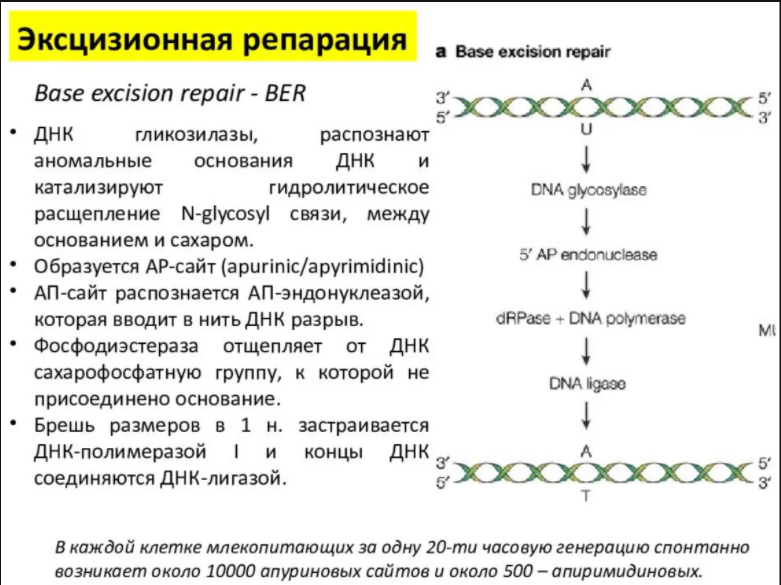
\includegraphics[width=0.8\linewidth]{10_BER}
	\caption{Эксцизионная репарация оснований (BER)}
	\label{fig:10_NER}
\end{figure}

\subsection{Эксцизионная репарация NER}

NER есть Nucleotide excision repair или \textbf{Эксцизионная репарация нуклеотидов}. Поврежденный нуклеотид узнается особым комплексом ферментов, вырезается и затем восстанавливается по исходной цепи. Механизм этого типа репарации представлен на рисунке \ref{fig:10_NER}.

\begin{figure}[H]
	\centering
	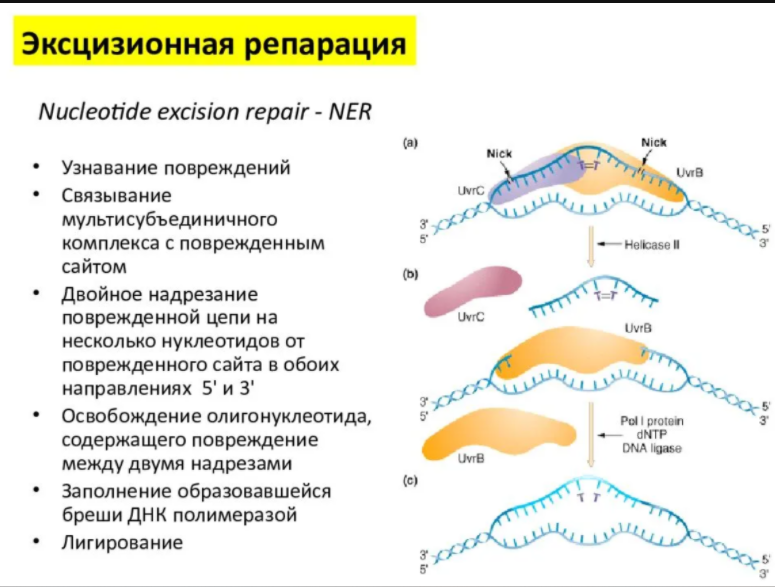
\includegraphics[width=0.8\linewidth]{10_NER}
	\caption{Эксцизионная репарация нуклеотидов (NER)}
	\label{fig:10_BER}
\end{figure}

\subsection{Белки эксцизионной репарации}

Тут так выходит что если прочитать все подряд, то получится NER у прокариот :)

\subsubsection{Гликозилаза}

Участвует в BER (с нее все начинается), распознает поврежденные основания, неспаренные основания и прочую гадость. После этого разрезает связь азотистого основания с дезоксирибозой, чем удаляет его из ДНК.

\subsubsection{АП-нуклеаза}

Катализирует разрыв внутренних фосфодиэфирных связей в одно-или двунитчатой молекуле ДНК.

\subsubsection{UvrABCD}

Эндонуклаза, образуемая белками UvrA, UvrB и UvrC (вообще все же обычно говорят о UvrABC) и действующей с ней хеликазы UvrD. Сначала UvrA распознает пиримидиновые димеры и прочие крупные повреждения, после чего связывается с UvrB, а дальше прикрепляется UvrC, который вносит надрезы в ДНК по обе стороны от повреждения. После этого хеликаза UvrD расплетает ДНК между насечками, благодаря чему поврежденная цепь высвобождается.

\subsubsection{ДНК-полимераза II}

Участвует в репарации поврежденной ДНК. Обладает способностью 5'-3'-удлинения цепочки и 3'-5'-экзонуклеазным действием и вот понимай как хочешь.

\subsection{SOS-ответ бактерий и роль всевозможных генов}

Сперва вообще скажем, что такое SOS-репарация. Это последняя возможность для ДНК, которая подошла к репликации, имея не устраненные повреждения, сохранить целостность. Если репликация на первом же не устраненном повреждении <<остановится>>, то клетка может погибнуть.  У человека мутации в генах этих белков вызывают наследственное заболевание --- синдром Кокэйна. В процессе эволюции сформировался крайне рискованный механизм репарации, названный <<SOS-репарация ДНК>>. Основная задача такой системы – пройти поврежденный участок ДНК таким образом, чтобы не блокировалось действие ДНК-полимеразы. В результате клетка спасается от гибели на данном этапе и может обеспечить митоз, хотя будут ошибки и высокий риск гибели клетки. Наиболее изучена SOS-репарация у Е.coli, ключевыми белками которой являются белки recA и lexА, поэтому будем смотреть их механизм.

Если в ДНК появляются летальные дефекты, блокирующие ДНК-полимеразу в процессе репликации (например, одноцепочечные разрывы, др.), в клетке активируется система SOS-репарации. Эта система состоит из нескольких десятков белков (recA, lexA, umuD, umuC и др.). В активном состоянии эти белки способствуют формированию полимеразы~V, для которой характерна низкая специфичность (сродство) к материнской цепи ДНК. Это свойство позволяет вставлять в дочернюю цепь нуклеотид, не комплементарный нуклеотиду материнской цепи, преодолевать место повреждения и продолжать процесс репликации. В неповрежденной ДНК активность генов, ответственных за синтез белков полимеразы V, блокируется белком lexA.

Одной из функций белка recA является включение генов umuD и umuC, которые способны замедлять процесс синтеза ДНК при наличии повреждений ДНК. Эти белки могут присоединяться к ДНК-полимеразе~III, снижая ее корректорские функции. Измененный репликационный комплекс продолжает синтез дочерней цепи ДНК на поврежденной матрице, подставляя нуклеотиды случайным образом. В результате дочерние цепи ДНК накапливают ошибки репликации напротив поврежденных нуклеотидов.

\subsubsection{Этапы SOS-репарации}

\begin{enumerate}
	\item В цепи ДНК формируется повреждение, которое ДНК-полимераза~III не может пройти и репликация останавливается. 
	
	\item Активируется синтез белка recA6. Этот белок взаимодействует с белком-репрессором LexA и способствует его аутопротеолизу (расщеплению белка под действием собственных ферментов). После этого и запускается синтез белков, способствующих SOS-репарации. (Начало SOS- ответа определяется взаимодействием белка RecA с белком репрессором LexA. Ответ клетки на повреждающее воздействие начинается с активации протеазной активности белка RecA. Активирующим сигналом может быть присутствие одноцепочечной области в сайте повреждения. Активируясь, RecA-протеаза разрезает белок-репрессор LexA. Белок LexA в неповрежденных клетках функционирует как репрессор многих оперонов, гены которых отвечают за различные репарационные функции. Протеолитическое разрезание репрессора (белка LexA) индуцирует все эти опероны. LexA связывает в своих мишенях так называемый SOS-бокс — участок длиной 20 пар оснований, содержащий консенсус из восьми абсолютно консервативных позиций. Как правило, SOS-бокс входит в состав промотора. LexA репрессирует также ген recA и собственный ген, поэтому в условиях SOS-ответа идёт активный синтез обоих белков. Уровень RecA может повыситься в 50 раз, и в таких концентрациях RecA начинает сам участвовать в эксцизионной репарации. При этом RecA продолжает индуцировать саморасщепление LexA, что не даёт ему функционировать в роли репрессора во время SOS-ответа)
	
	\item Вновьсинтезированный белок RecA закручивается спиралью вокруг одноцепочечной ДНК для ее стабилизации.
	
	\item Активируется синтез белков UmuD, UmuC и прочих.
	
	\item синтезированные белки UmuD и UmuC соединяются со спиралью RecA и образуют комплекс. Основная задача этого комплекса – <<проскочить>> сложный дефект без формирования бреши напротив дефекта. После привлечения комплекса он вытесняет один из структурных компонентов ДНК-полимеразы~III и занимает его место, начиная полимеризацию случайных нуклеотидов на поврежденной матрице. В результате возрастает выживаемость клетки (SOS-репарация) и создаются условия для возникновения мутации (SOS-мутагенез).
	
	\item После прохождения дефектного участка полимераза V отсоединяется от цепи ДНК и работу возобновляет полимераза~III.
\end{enumerate}

Интенсивность SOS-ответа клетки зависит от степени повреждения ДНК, так как только большое количество однонитевой ДНК позволяет активироваться RecA белку в количестве, достаточном для открытия SOS-регулона. Так как белок RecA связывается c LexA в том же сайте, в котором происходит его связывание с двунитевой ДНК, то при запуске SOS-ответа белок RecA не активирует процесс гомологической рекомбинации. В норме при гомологичной рекомбинации SOS-ответ также выражен слабо.

\begin{figure}[H]
	\centering
	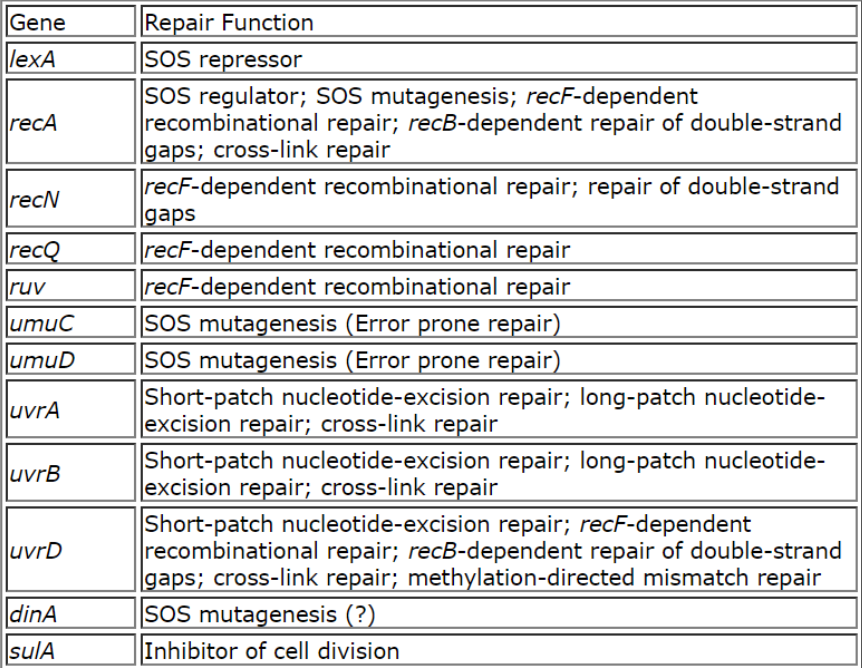
\includegraphics[width=0.7\linewidth]{10_gene_functions}
	\caption{Гены и их функции}
\end{figure}

\subsubsection{uvrABCD}

Эндонуклеаза UvrABC представляет собой мультиферментный комплекс в бактериях, участвующих в репарации ДНК путем эксцизионной репарации нуклеотидов, и поэтому ее иногда называют эксинуклеазой. Этот процесс восстановления UvrABC, иногда называемый процессом короткого участка, включает удаление двенадцати нуклеотидов, где произошла генетическая мутация, с последующей ДНК-полимеразой, замена этих аберрантных нуклеотидов правильными нуклеотидами и завершение восстановления ДНК. Субъединицы для этого фермента кодируются в генах uvrA, uvrB и uvrC. Этот ферментный комплекс способен восстанавливать многие виды повреждений, в том числе образование циклобутилдимера.

Как это происходит?

\begin{enumerate}
	\item Два белка UvrA образуют димер, и оба они имеют АТФазную / ГТФазную активность.
	
	\item Димер UvrA связывается с димером UvrB и образует комплекс, способный обнаруживать повреждение ДНК. Димер UvrA функционирует как единица, ответственная за обнаружение повреждения ДНК, вероятно, посредством механизма обнаружения искажений в двойной спирали ДНК.
	
	\item После связывания комплекса UvrA2B2 с предполагаемым поврежденным участком ДНК оборачивается вокруг UvrB.
	
	\item Димер UvrA уходит, и белок UvrC входит и связывается с UvrB и, следовательно, образует новый комплекс UvrBC.
	
	\item UvrC отвечает за расщепление нуклеотидов с обеих сторон повреждения ДНК. Он расщепляет фосфодиэфирную связь на четыре нуклеотида после повреждения ДНК, и расщепляет фосфодиэфирную связь на восемь нуклеотидов выше повреждения ДНК и создает отрезанный из двенадцати нуклеотидов сегмент.
	
	\item Затем вступает ДНК геликаза~II (иногда называемая \textbf{UvrD}) и удаляет вырезанный сегмент, удаляя спаривание оснований. UvrB все еще остается на месте, даже несмотря на то, что UvrC на этом этапе диссоциировал, так как UvrB может быть вовлечен для предотвращения повторного отжига вырезанной ДНК.
	
	\item Входит ДНК-полимераза~I и заполняет правильную нуклеотидную последовательность, отсекая при этом UvrB, и последняя фосфодиэфирная связь завершается с помощью ДНК-лигазы.
\end{enumerate}
